% !TEX root = top.tex
\subsection{Anytime Prediction}
In the real-time setting, the computational budget available can vary for each test case and cannot
be known ahead of time. This is formalized in anytime prediction, \citep{grubb2012speedboost}  the
setting in which for each test example $\rvx$, there is non-deterministic computational budget $B$
drawn from the joint distribution $P(\rvx, B)$. The goal is then to minimize the expected loss $L(f)
= \E\left[ L\left( f(\rvx), B \right)\right]_{P(\rvx, B)}$, where $f(\cdot)$ is the model and
$L(\cdot)$ is the loss for an $f(\cdot)$ that must produce a prediction within the budget $B$.

We conduct experiments on CIFAR-10. Our anytime search space consists of networks with 3 cells
containing 24, 16, and 8 nodes. Each node is given the additional properties: 1) the spatial size it
operates at and 2) if an early-exit classifier is attached to it. A node enforces its spatial size
by pooling or upsampling any input feature maps inputs that are of different scale. Note that while
a naive one-shot model would triple its size to include three different parameter sets at three
different scales, the GHN is negligibly affected by such a change. The GHN uses the area under the
predicted accuracy-FLOPS curve as its selection criteria. The search space, contains various
convolution and pooling operators. Training methodology of the final architectures are chosen to
match \cite{huang2017multi} and can be found in the Appendix.

Figure \ref{fig:test1} shows a comparison with the various methods presented by
\cite{huang2017multi}. Our experiments show that the best searched architectures can outperform the
current state-of-the-art human designed networks. We see the GHN is amenable to the changes proposed
above, and can find efficient architectures with a random search when used with a strong search
space.

\iflatexml
\begin{figure}
  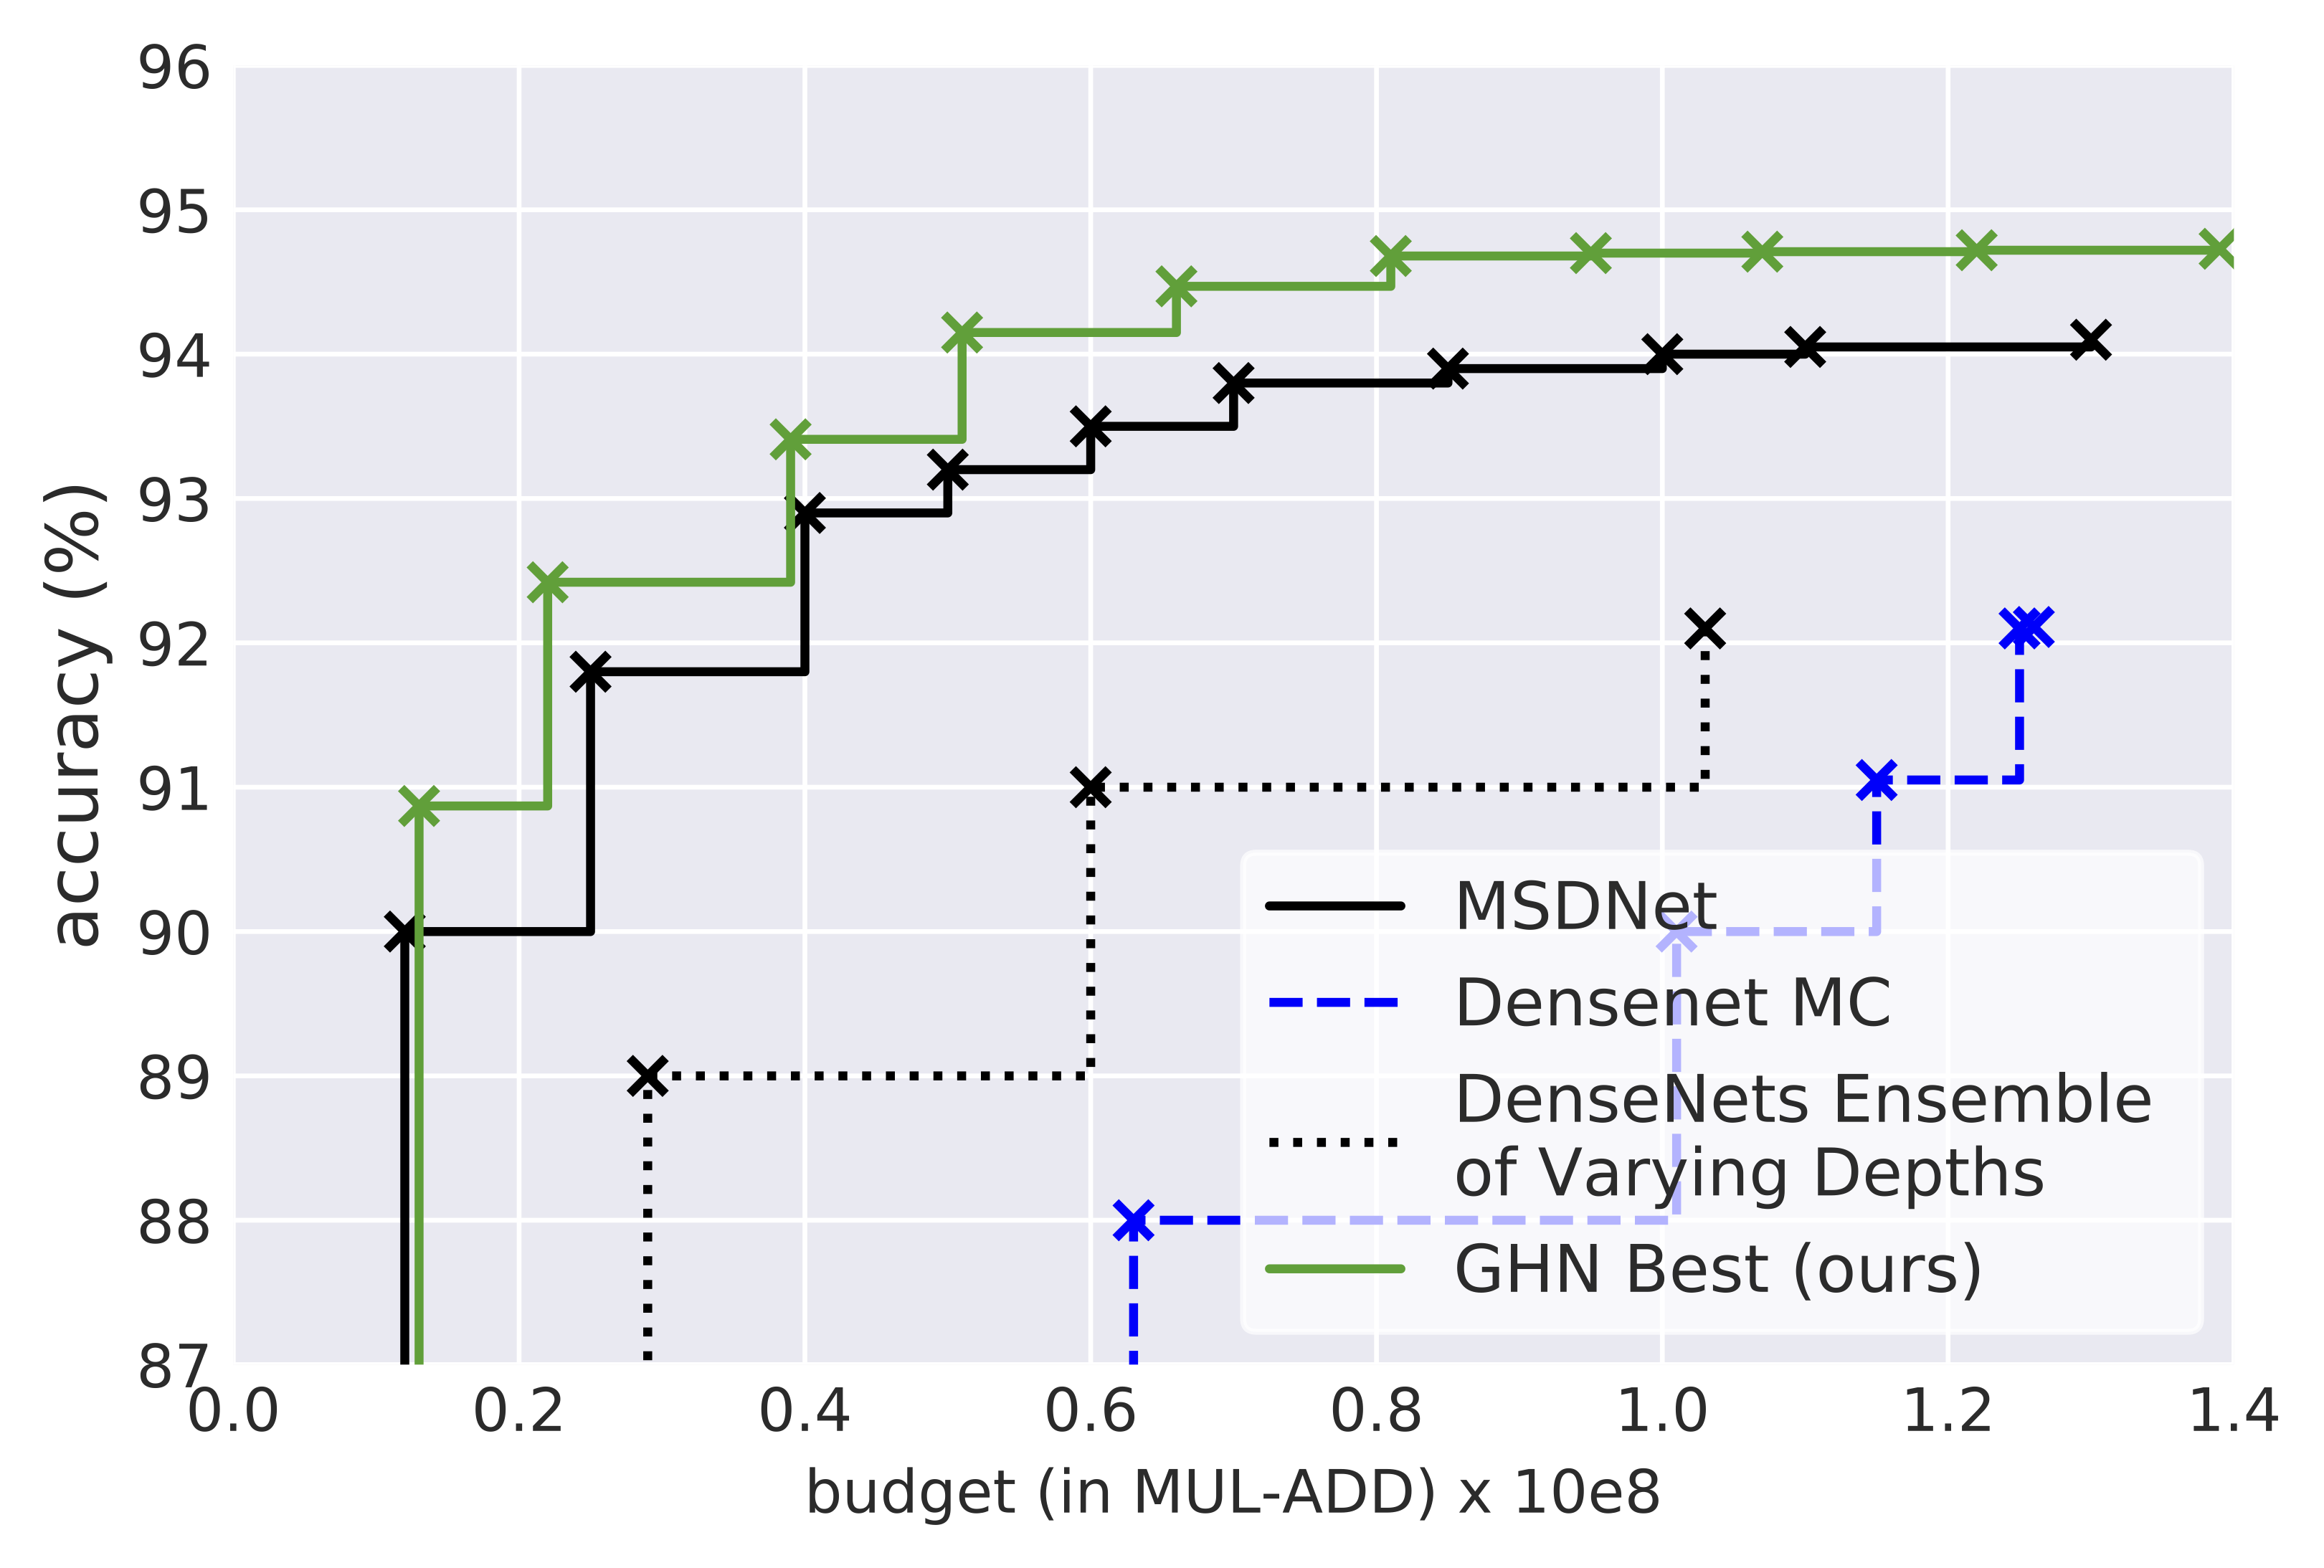
\includegraphics[width=4\linewidth]{figures/anytime_compare.png}
  \captionof{figure}{Comparison with state-of-the-art\\ human-designed networks on CIFAR-10.}
  \label{fig:test1}
\end{figure}
\begin{figure}
  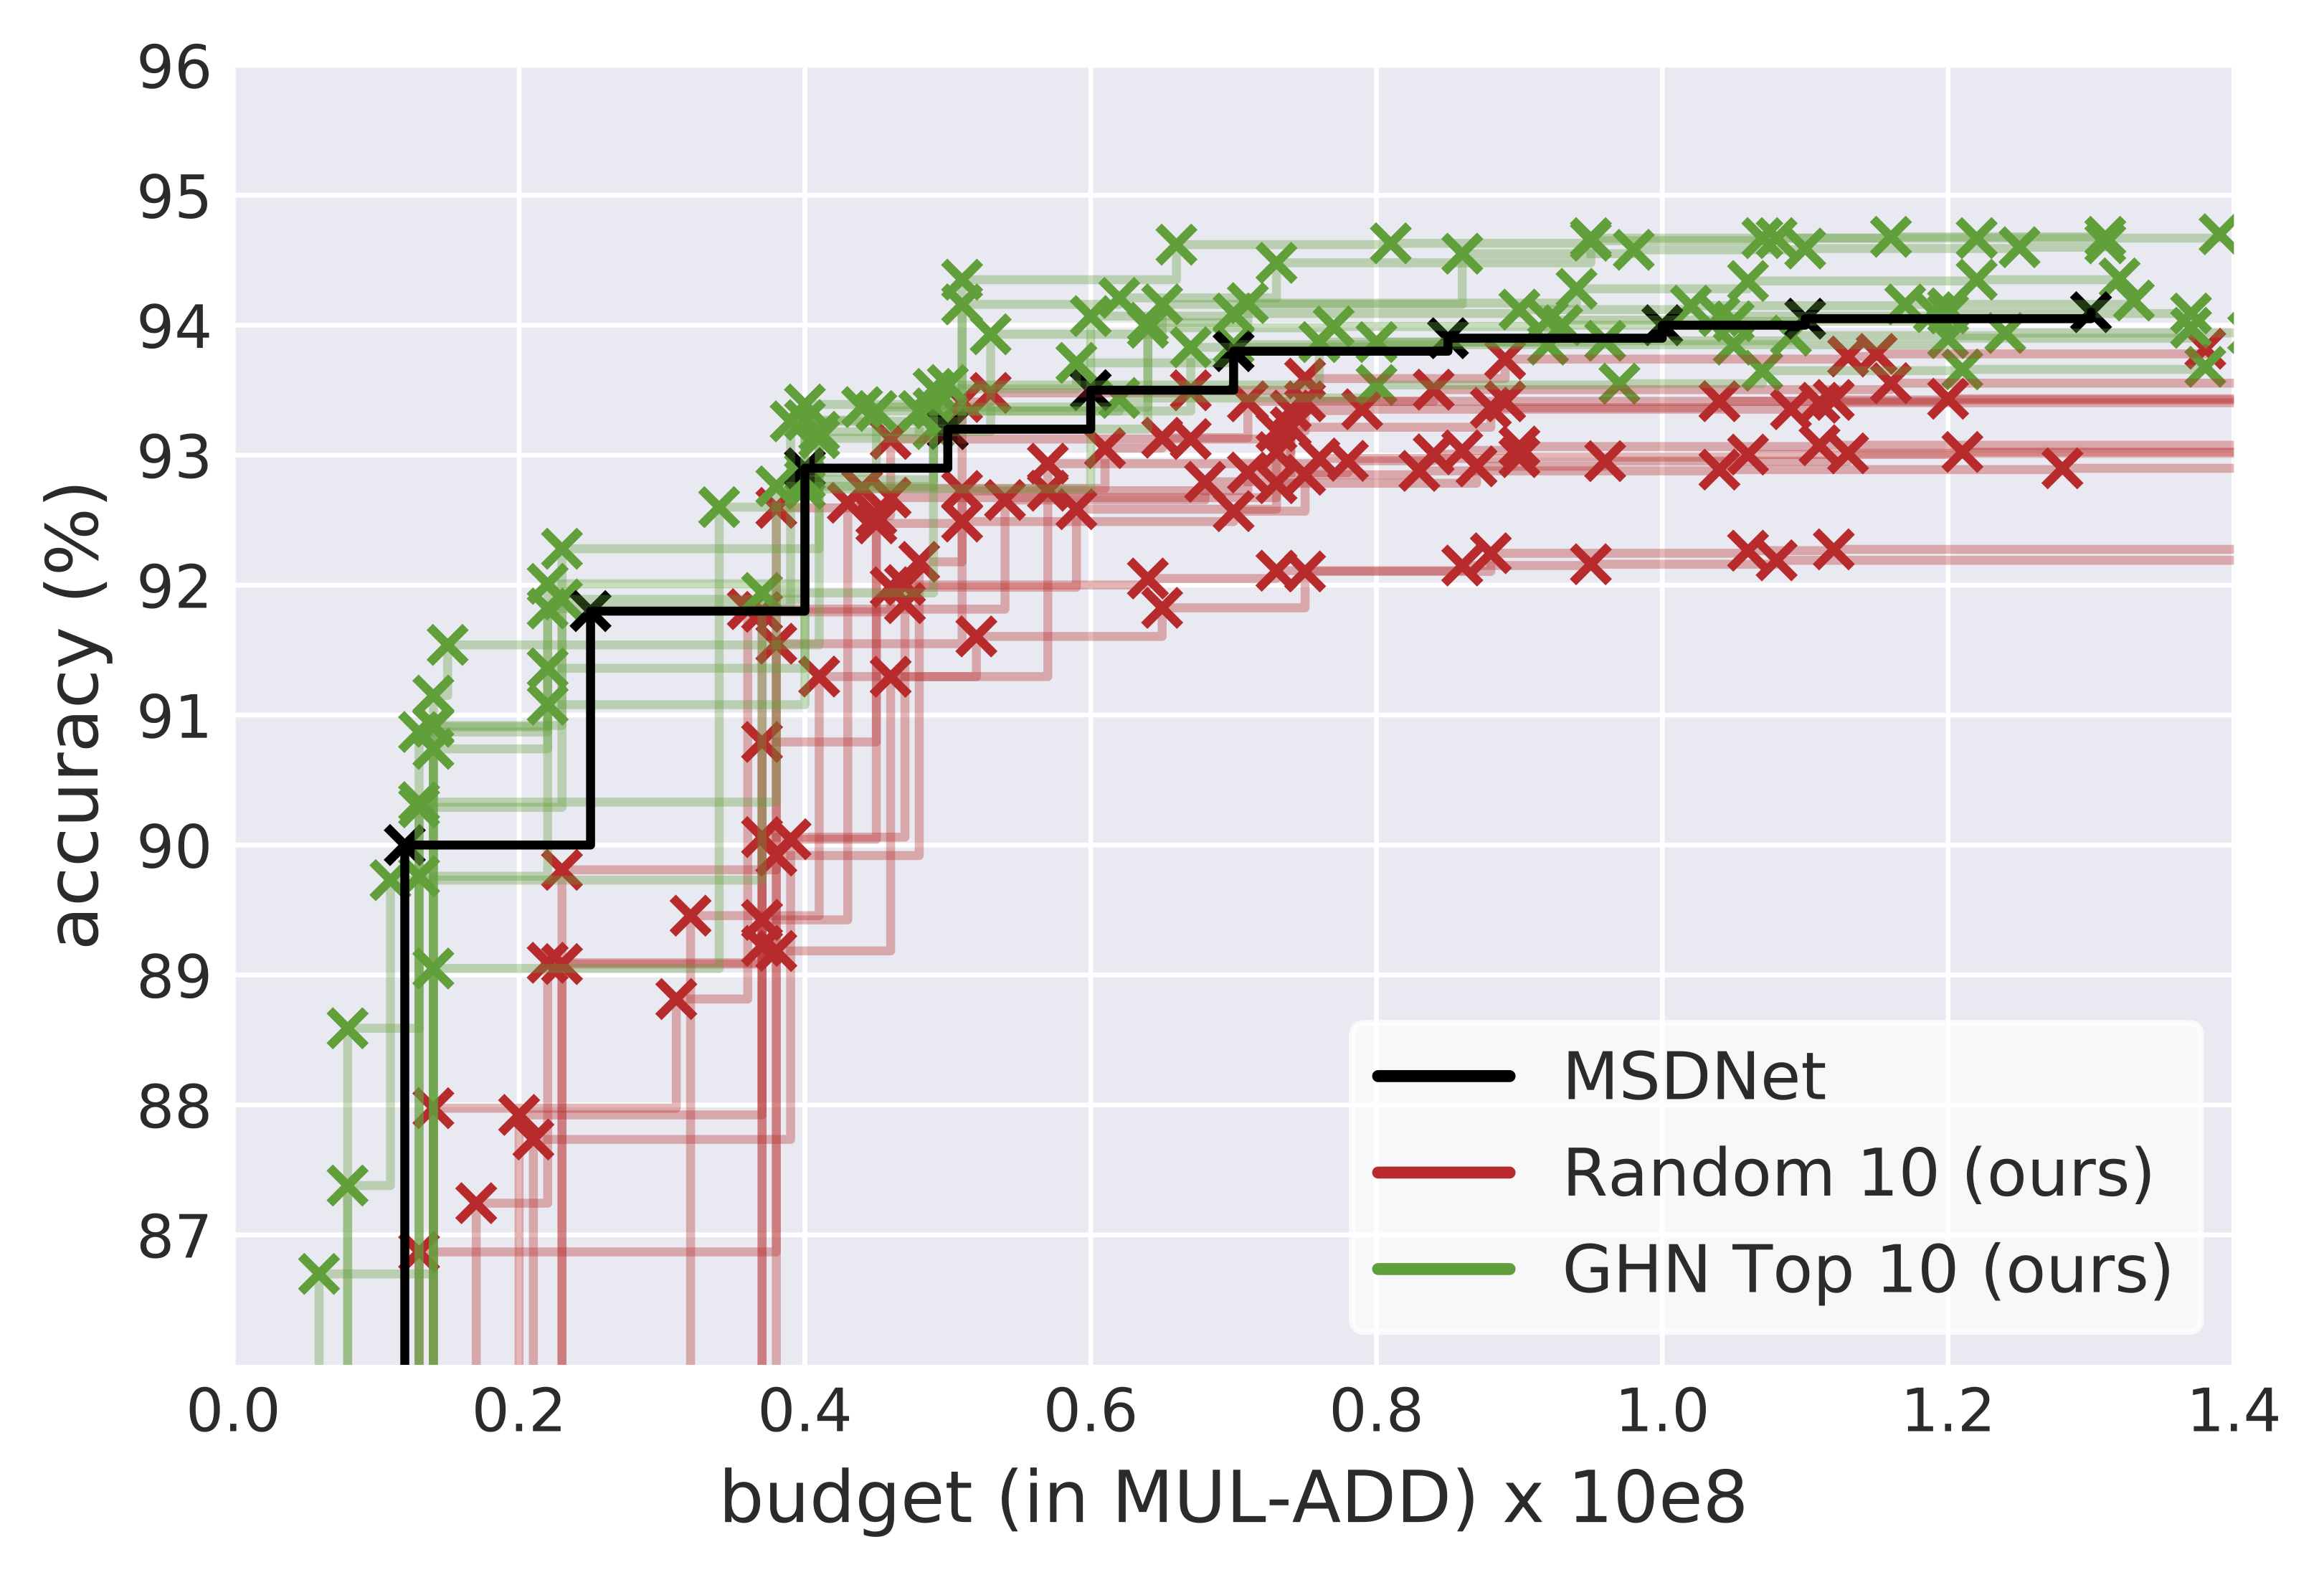
\includegraphics[width=4\linewidth]{figures/anytime_randoms.png}
  \captionof{figure}{Comparison between random 10 and\\ top 10 networks on CIFAR-10.}
  \label{fig:test2}
\end{figure}
\else
\begin{figure}[t]
\vspace{-0.5cm}
\centering
\begin{minipage}{.48\textwidth}
  \centering
  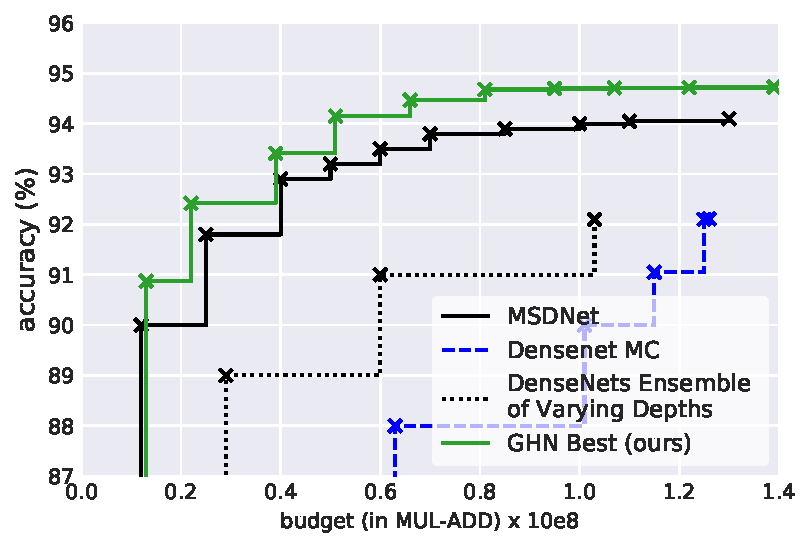
\includegraphics[width=0.8\linewidth]{figures/anytime_compare.pdf}
  \captionof{figure}{Comparison with state-of-the-art\\ human-designed networks on CIFAR-10.}
\label{table:Results4}
  \label{fig:test1}
\end{minipage}%
\begin{minipage}{.48\textwidth}
  \centering
  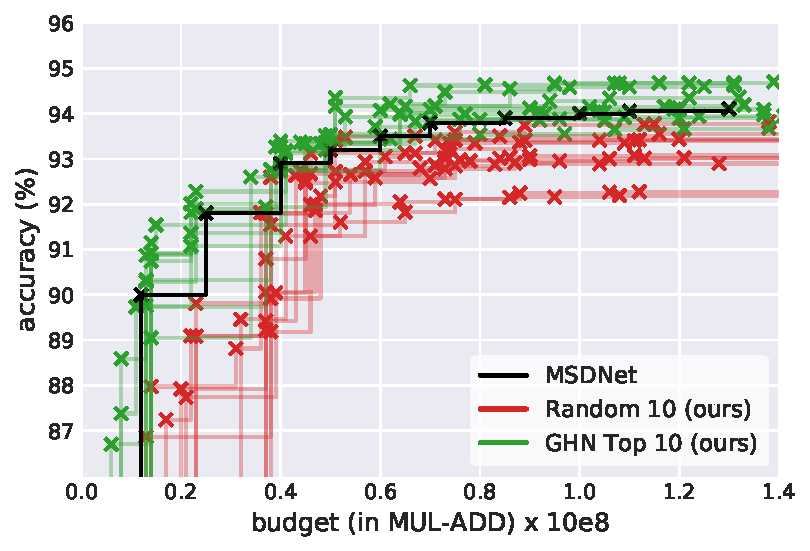
\includegraphics[width=0.8\linewidth]{figures/anytime_randoms.pdf}
  \captionof{figure}{Comparison between random 10 and\\ top 10 networks on CIFAR-10.}
  \label{fig:test2}
\end{minipage}
\end{figure}
\fi